\documentclass{article}
\usepackage[utf8]{inputenc}
\usepackage{tikz}

\begin{document}

\section{Original copy}
\centering
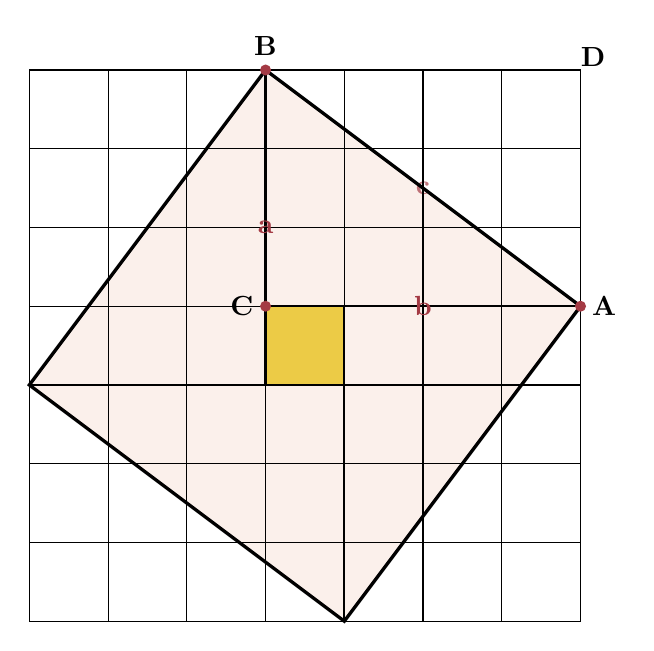
\begin{tikzpicture}
% Colors define
\definecolor{myRed}{HTML}{A43A44}
\definecolor{myOrange}{HTML}{F9EAE3}
\definecolor{myYellow}{HTML}{ECCB46}

% Important positions
\node (A) at (7,4) {};
\node (B) at (3,7) {};
\node (C) at (3,4) {};
\node (D) at (7,7) {};

% Big rectangle color
\fill[myOrange,opacity=0.7] (4,0) -- (0,3) -- (B.center) -- (A.center) node[midway,myRed]{\textbf{c}} -- cycle;

% Here we draw the grid and te colored square
\fill[myYellow] (3,3) rectangle (4,4);
\draw[] (0,0) grid (7,7);

% Big rectangle
\draw[very thick] (4,0) -- (0,3) -- (B.center) -- (A.center) -- cycle;

% Position labels
\node at (A.east) [xshift=5] {\textbf{A}};
\node at (B.north) [yshift=5] {\textbf{B}};
\node at (C.west) [xshift=-5] {\textbf{C}};
\node at (D.north east) [xshift=1,yshift=1] {\textbf{D}};

% Thicker lines of the box
\draw[thick] (C.center) -- (A.center) node[midway,myRed]{\textbf{b}};
\draw[thick] (3,3) -- (B.center) node[midway,myRed]{\textbf{a}};
\draw[thick] (4,3) -- (0,3);
\draw[thick] (4,4) -- (4,0);

% Circles
\foreach \n in {A,B,C}
    \fill[myRed] (\n.center) circle[radius=0.07];
\end{tikzpicture}

\section{My version}
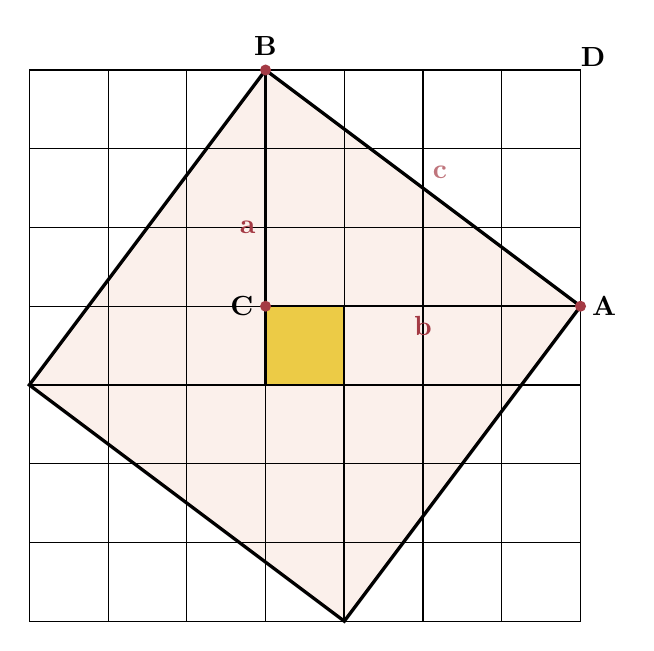
\begin{tikzpicture}
% Colors define
\definecolor{myRed}{HTML}{A43A44}
\definecolor{myOrange}{HTML}{F9EAE3}
\definecolor{myYellow}{HTML}{ECCB46}

% Important positions
\node (A) at (7,4) {};
\node (B) at (3,7) {};
\node (C) at (3,4) {};
\node (D) at (7,7) {};

% Big rectangle color
\fill[myOrange,opacity=0.7] (4,0) -- (0,3) -- (B.center) to[] node[auto,myRed]{\textbf{c}} (A.center) -- cycle;

% Here we draw the grid and te colored square
\fill[myYellow] (3,3) rectangle (4,4);
\draw[] (0,0) grid (7,7);

% Big rectangle
\draw[very thick] (4,0) -- (0,3) -- (B.center) -- (A.center) -- cycle;

% Position labels
\node at (A.east) [xshift=5] {\textbf{A}};
\node at (B.north) [yshift=5] {\textbf{B}};
\node at (C.west) [xshift=-5] {\textbf{C}};
\node at (D.north east) [xshift=1,yshift=1] {\textbf{D}};

% Thicker lines of the box
\draw[thick] (C.center) to[] node[auto,swap,myRed]{\textbf{b}} (A.center);
\draw[thick] (3,3) to[] node[auto,myRed]{\textbf{a}} (B.center);
\draw[thick] (4,3) -- (0,3);
\draw[thick] (4,4) -- (4,0);

% Circles
\foreach \n in {A,B,C}
    \fill[myRed] (\n.center) circle[radius=0.07];
\end{tikzpicture}

\end{document}
